\documentclass[10pt]{article}
\usepackage[T1]{fontenc}
\usepackage{lmodern}
\usepackage{mathtools}
\usepackage{booktabs}
\usepackage{adjustbox}
\usepackage[left=1.5cm, right=2cm, top=1.5cm, bottom=2cm]{geometry}
\usepackage{tikz}
\usepackage{pgfplots}
\pgfplotsset{compat=1.18}
\usetikzlibrary{arrows.meta,positioning,calc}
\setlength\parindent{0pt}
\title{g7 1 - Shared Protection - Custom Algorithm - Ascending}
\date{}
\author{}

\begin{document}
\maketitle
\section*{Topology}
\begin{center}\begin{adjustbox}{max width=\linewidth}
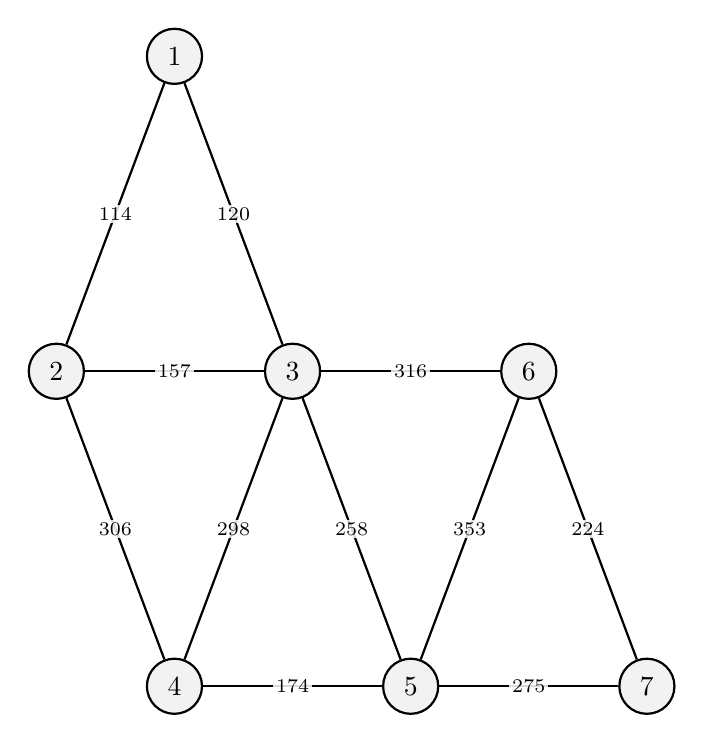
\begin{tikzpicture}[baseline, >={Stealth[length=2mm]},
  netnode/.style={circle, draw, thick, fill=gray!10, minimum size=7mm, inner sep=1pt},
  link/.style={thick},
  linklabel/.style={font=\scriptsize, inner sep=1pt, fill=white, fill opacity=0.85, text opacity=1}]
\node[netnode] (S1) at (1.500,8.000) {1};
\node[netnode] (S2) at (0.000,4.000) {2};
\node[netnode] (S3) at (3.000,4.000) {3};
\node[netnode] (S4) at (1.500,0.000) {4};
\node[netnode] (S5) at (4.500,0.000) {5};
\node[netnode] (S6) at (6.000,4.000) {6};
\node[netnode] (S7) at (7.500,0.000) {7};
\draw[link] (S1) to node[linklabel] {114} (S2);
\draw[link] (S1) to node[linklabel] {120} (S3);
\draw[link] (S2) to node[linklabel] {157} (S3);
\draw[link] (S2) to node[linklabel] {306} (S4);
\draw[link] (S3) to node[linklabel] {298} (S4);
\draw[link] (S3) to node[linklabel] {258} (S5);
\draw[link] (S3) to node[linklabel] {316} (S6);
\draw[link] (S4) to node[linklabel] {174} (S5);
\draw[link] (S5) to node[linklabel] {353} (S6);
\draw[link] (S5) to node[linklabel] {275} (S7);
\draw[link] (S6) to node[linklabel] {224} (S7);
\end{tikzpicture}
\end{adjustbox}\end{center}
\section*{Performance Parameters}
\begin{center}\begin{tabular}{lr}
\toprule
Highest link load & 73 Gb/s \\
Highest used FSU & 119 / 320 \\
Total used FSUs & 117 \\
Transponder cost & 58.5 \\
\midrule
SC-DP-QPSK transponders & 39 \\
SC-DP-16QAM transponders & 0 \\
DP-16QAM transponders & 0 \\
\bottomrule
\end{tabular}\end{center}
\clearpage
\section*{Link Load Map}
\begin{center}\begin{adjustbox}{max width=\linewidth}
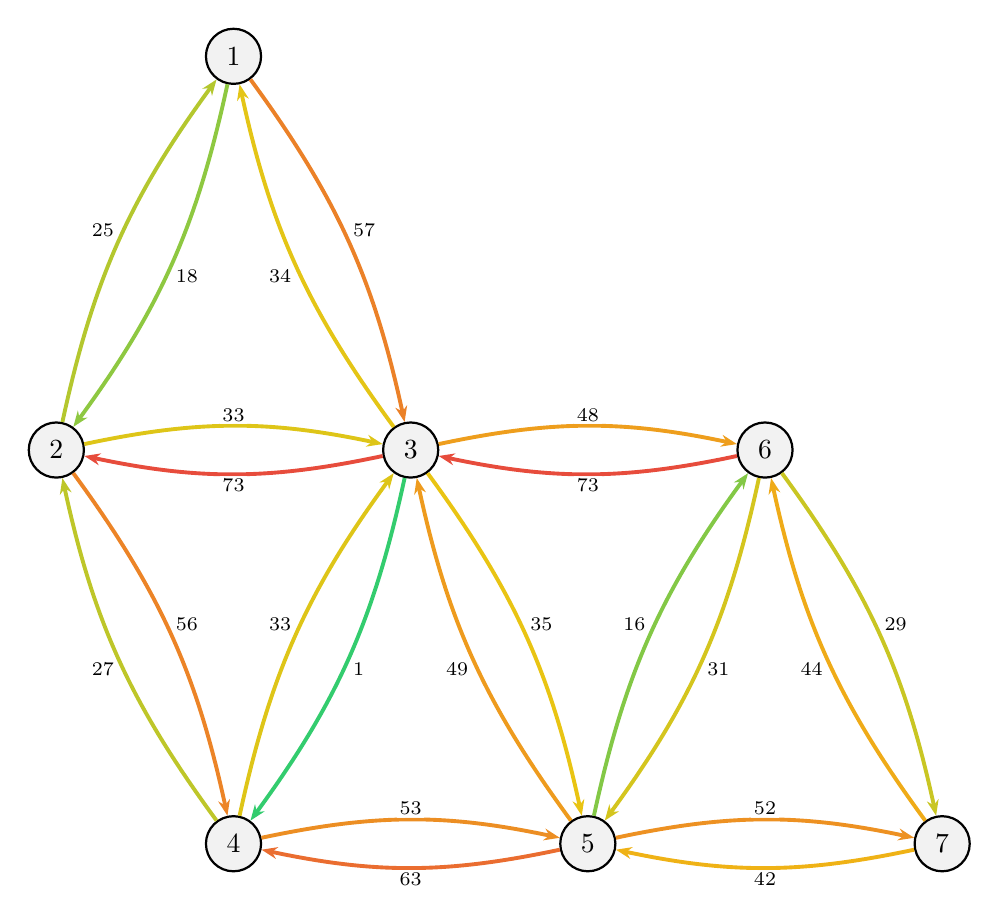
\begin{tikzpicture}[baseline, >={Stealth[length=2mm]},
  netnode/.style={circle, draw, thick, fill=gray!10, minimum size=7mm, inner sep=1pt},
  link/.style={line width=1.4pt},
  linklabel/.style={font=\scriptsize, inner sep=1pt, fill=white, fill opacity=0.85, text opacity=1}]
\node[netnode] (S1) at (2.250,10.000) {1};
\node[netnode] (S2) at (0.000,5.000) {2};
\node[netnode] (S3) at (4.500,5.000) {3};
\node[netnode] (S4) at (2.250,0.000) {4};
\node[netnode] (S5) at (6.750,0.000) {5};
\node[netnode] (S6) at (9.000,5.000) {6};
\node[netnode] (S7) at (11.250,0.000) {7};
\draw[link, ->, draw={rgb,255:red,142;green,200;blue,65}] (S1) to[bend left=12] node[linklabel, auto] {18} (S2);
\draw[link, ->, draw={rgb,255:red,235;green,129;blue,40}] (S1) to[bend left=12] node[linklabel, auto] {57} (S3);
\draw[link, ->, draw={rgb,255:red,180;green,199;blue,46}] (S2) to[bend left=12] node[linklabel, auto] {25} (S1);
\draw[link, ->, draw={rgb,255:red,222;green,197;blue,24}] (S2) to[bend left=12] node[linklabel, auto] {33} (S3);
\draw[link, ->, draw={rgb,255:red,236;green,132;blue,39}] (S2) to[bend left=12] node[linklabel, auto] {56} (S4);
\draw[link, ->, draw={rgb,255:red,228;green,197;blue,22}] (S3) to[bend left=12] node[linklabel, auto] {34} (S1);
\draw[link, ->, draw={rgb,255:red,231;green,76;blue,60}] (S3) to[bend left=12] node[linklabel, auto] {73} (S2);
\draw[link, ->, draw={rgb,255:red,51;green,204;blue,110}] (S3) to[bend left=12] node[linklabel, auto] {1} (S4);
\draw[link, ->, draw={rgb,255:red,233;green,196;blue,19}] (S3) to[bend left=12] node[linklabel, auto] {35} (S5);
\draw[link, ->, draw={rgb,255:red,238;green,158;blue,29}] (S3) to[bend left=12] node[linklabel, auto] {48} (S6);
\draw[link, ->, draw={rgb,255:red,190;green,198;blue,41}] (S4) to[bend left=12] node[linklabel, auto] {27} (S2);
\draw[link, ->, draw={rgb,255:red,222;green,197;blue,24}] (S4) to[bend left=12] node[linklabel, auto] {33} (S3);
\draw[link, ->, draw={rgb,255:red,236;green,142;blue,35}] (S4) to[bend left=12] node[linklabel, auto] {53} (S5);
\draw[link, ->, draw={rgb,255:red,238;green,155;blue,30}] (S5) to[bend left=12] node[linklabel, auto] {49} (S3);
\draw[link, ->, draw={rgb,255:red,234;green,109;blue,48}] (S5) to[bend left=12] node[linklabel, auto] {63} (S4);
\draw[link, ->, draw={rgb,255:red,131;green,200;blue,70}] (S5) to[bend left=12] node[linklabel, auto] {16} (S6);
\draw[link, ->, draw={rgb,255:red,237;green,145;blue,34}] (S5) to[bend left=12] node[linklabel, auto] {52} (S7);
\draw[link, ->, draw={rgb,255:red,231;green,76;blue,60}] (S6) to[bend left=12] node[linklabel, auto] {73} (S3);
\draw[link, ->, draw={rgb,255:red,212;green,197;blue,30}] (S6) to[bend left=12] node[linklabel, auto] {31} (S5);
\draw[link, ->, draw={rgb,255:red,201;green,198;blue,35}] (S6) to[bend left=12] node[linklabel, auto] {29} (S7);
\draw[link, ->, draw={rgb,255:red,239;green,178;blue,22}] (S7) to[bend left=12] node[linklabel, auto] {42} (S5);
\draw[link, ->, draw={rgb,255:red,239;green,171;blue,24}] (S7) to[bend left=12] node[linklabel, auto] {44} (S6);
\end{tikzpicture}
\end{adjustbox}\end{center}
\begin{center}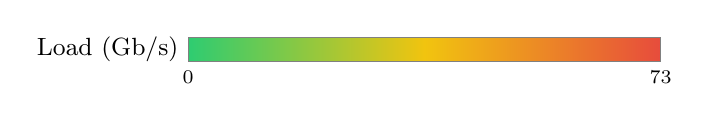
\begin{tikzpicture}
\definecolor{scalelow}{RGB}{46,204,113}\definecolor{scalemid}{RGB}{241,196,15}\definecolor{scalehigh}{RGB}{231,76,60}
\shade[left color=scalelow, right color=scalemid] (0,0) rectangle (3,0.3);
\shade[left color=scalemid, right color=scalehigh] (3,0) rectangle (6,0.3);
\draw[gray] (0,0) rectangle (6,0.3);
\node[below, font=\scriptsize] at (0,0) {0};
\node[below, font=\scriptsize] at (6,0) {73};
\node[left, font=\small] at (0,0.15) {Load (Gb/s)};
\end{tikzpicture}\end{center}
\section*{Link Load Distribution}

\begin{center}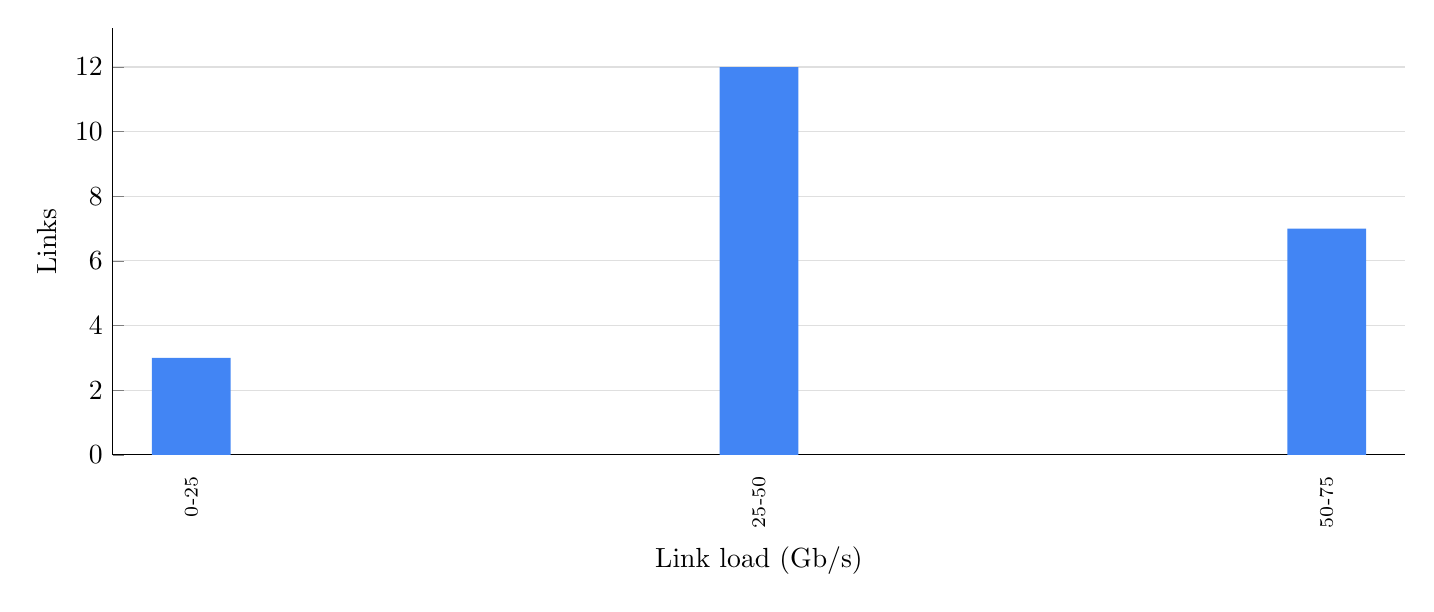
\begin{tikzpicture}
\begin{axis}[
  ybar, bar width=1.000cm, width=18.000cm, height=7cm,
  ymin=0, ymajorgrids, grid style={gray!25}, axis lines*=left,
  enlarge x limits={abs=1.000cm}, xtick=data, major x tick style={draw=none},
  x tick label style={rotate=90, font=\scriptsize, /pgf/number format/1000 sep=},
  legend style={at={(0.5,-0.3)}, anchor=north, legend columns=-1, draw=none},
  ylabel={Links},
  xlabel={Link load (Gb/s)},
  symbolic x coords={0-25,25-50,50-75}]
\addplot[fill={rgb,255:red,66;green,133;blue,244}, draw=none] coordinates {(0-25,3.000) (25-50,12.000) (50-75,7.000) };
\end{axis}
\end{tikzpicture}\end{center}
\clearpage
\section*{Spectrum Occupancy}
\begin{center}\begin{adjustbox}{max width=\linewidth}
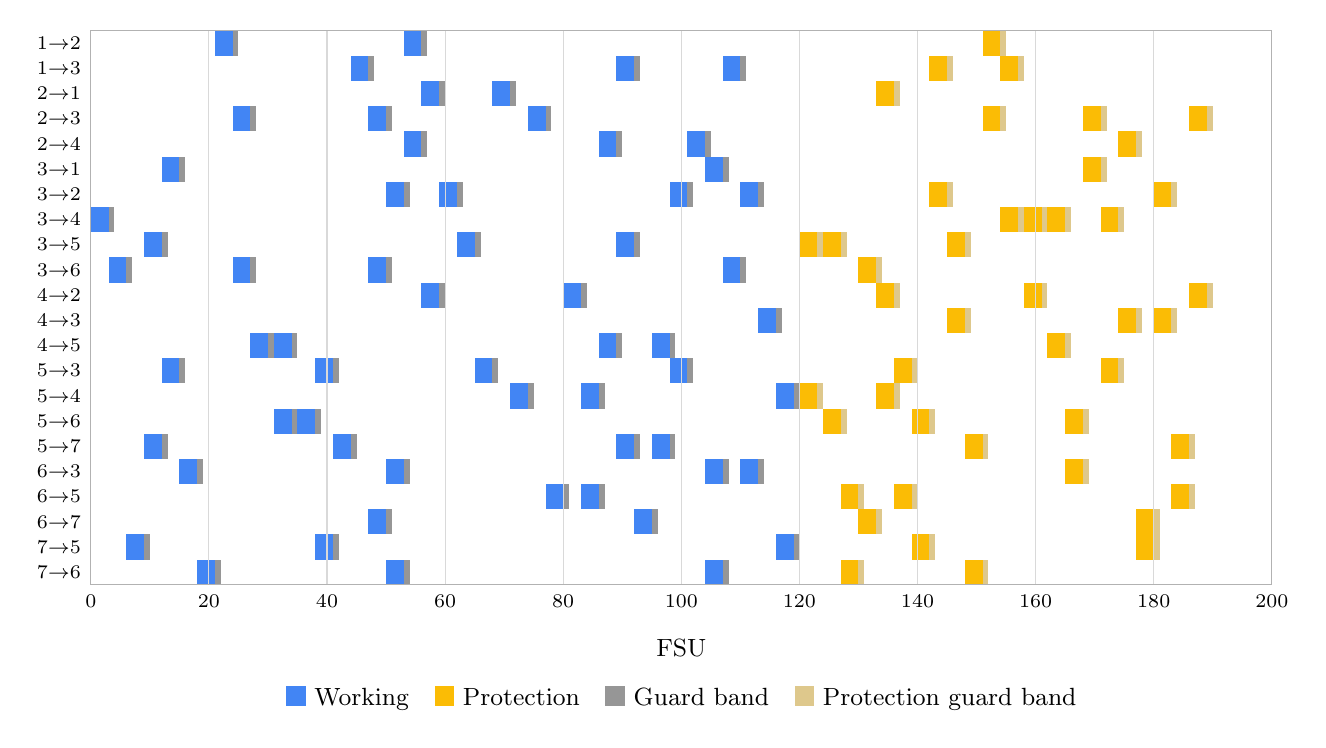
\begin{tikzpicture}[x=0.0750cm, y=-0.32cm]
\fill[fill={rgb,255:red,66;green,133;blue,244}] (21,0) rectangle (24,1);
\fill[fill={rgb,255:red,150;green,150;blue,150}] (24,0) rectangle (25,1);
\fill[fill={rgb,255:red,66;green,133;blue,244}] (53,0) rectangle (56,1);
\fill[fill={rgb,255:red,150;green,150;blue,150}] (56,0) rectangle (57,1);
\fill[fill={rgb,255:red,251;green,188;blue,5}] (151,0) rectangle (154,1);
\fill[fill={rgb,255:red,222;green,200;blue,140}] (154,0) rectangle (155,1);
\node[left, font=\scriptsize] at (0,0.5) {1\(\to\)2};
\fill[fill={rgb,255:red,66;green,133;blue,244}] (44,1) rectangle (47,2);
\fill[fill={rgb,255:red,150;green,150;blue,150}] (47,1) rectangle (48,2);
\fill[fill={rgb,255:red,66;green,133;blue,244}] (89,1) rectangle (92,2);
\fill[fill={rgb,255:red,150;green,150;blue,150}] (92,1) rectangle (93,2);
\fill[fill={rgb,255:red,66;green,133;blue,244}] (107,1) rectangle (110,2);
\fill[fill={rgb,255:red,150;green,150;blue,150}] (110,1) rectangle (111,2);
\fill[fill={rgb,255:red,251;green,188;blue,5}] (142,1) rectangle (145,2);
\fill[fill={rgb,255:red,222;green,200;blue,140}] (145,1) rectangle (146,2);
\fill[fill={rgb,255:red,251;green,188;blue,5}] (154,1) rectangle (157,2);
\fill[fill={rgb,255:red,222;green,200;blue,140}] (157,1) rectangle (158,2);
\node[left, font=\scriptsize] at (0,1.5) {1\(\to\)3};
\fill[fill={rgb,255:red,66;green,133;blue,244}] (56,2) rectangle (59,3);
\fill[fill={rgb,255:red,150;green,150;blue,150}] (59,2) rectangle (60,3);
\fill[fill={rgb,255:red,66;green,133;blue,244}] (68,2) rectangle (71,3);
\fill[fill={rgb,255:red,150;green,150;blue,150}] (71,2) rectangle (72,3);
\fill[fill={rgb,255:red,251;green,188;blue,5}] (133,2) rectangle (136,3);
\fill[fill={rgb,255:red,222;green,200;blue,140}] (136,2) rectangle (137,3);
\node[left, font=\scriptsize] at (0,2.5) {2\(\to\)1};
\fill[fill={rgb,255:red,66;green,133;blue,244}] (24,3) rectangle (27,4);
\fill[fill={rgb,255:red,150;green,150;blue,150}] (27,3) rectangle (28,4);
\fill[fill={rgb,255:red,66;green,133;blue,244}] (47,3) rectangle (50,4);
\fill[fill={rgb,255:red,150;green,150;blue,150}] (50,3) rectangle (51,4);
\fill[fill={rgb,255:red,66;green,133;blue,244}] (74,3) rectangle (77,4);
\fill[fill={rgb,255:red,150;green,150;blue,150}] (77,3) rectangle (78,4);
\fill[fill={rgb,255:red,251;green,188;blue,5}] (151,3) rectangle (154,4);
\fill[fill={rgb,255:red,222;green,200;blue,140}] (154,3) rectangle (155,4);
\fill[fill={rgb,255:red,251;green,188;blue,5}] (168,3) rectangle (171,4);
\fill[fill={rgb,255:red,222;green,200;blue,140}] (171,3) rectangle (172,4);
\fill[fill={rgb,255:red,251;green,188;blue,5}] (186,3) rectangle (189,4);
\fill[fill={rgb,255:red,222;green,200;blue,140}] (189,3) rectangle (190,4);
\node[left, font=\scriptsize] at (0,3.5) {2\(\to\)3};
\fill[fill={rgb,255:red,66;green,133;blue,244}] (53,4) rectangle (56,5);
\fill[fill={rgb,255:red,150;green,150;blue,150}] (56,4) rectangle (57,5);
\fill[fill={rgb,255:red,66;green,133;blue,244}] (86,4) rectangle (89,5);
\fill[fill={rgb,255:red,150;green,150;blue,150}] (89,4) rectangle (90,5);
\fill[fill={rgb,255:red,66;green,133;blue,244}] (101,4) rectangle (104,5);
\fill[fill={rgb,255:red,150;green,150;blue,150}] (104,4) rectangle (105,5);
\fill[fill={rgb,255:red,251;green,188;blue,5}] (174,4) rectangle (177,5);
\fill[fill={rgb,255:red,222;green,200;blue,140}] (177,4) rectangle (178,5);
\node[left, font=\scriptsize] at (0,4.5) {2\(\to\)4};
\fill[fill={rgb,255:red,66;green,133;blue,244}] (12,5) rectangle (15,6);
\fill[fill={rgb,255:red,150;green,150;blue,150}] (15,5) rectangle (16,6);
\fill[fill={rgb,255:red,66;green,133;blue,244}] (104,5) rectangle (107,6);
\fill[fill={rgb,255:red,150;green,150;blue,150}] (107,5) rectangle (108,6);
\fill[fill={rgb,255:red,251;green,188;blue,5}] (168,5) rectangle (171,6);
\fill[fill={rgb,255:red,222;green,200;blue,140}] (171,5) rectangle (172,6);
\node[left, font=\scriptsize] at (0,5.5) {3\(\to\)1};
\fill[fill={rgb,255:red,66;green,133;blue,244}] (50,6) rectangle (53,7);
\fill[fill={rgb,255:red,150;green,150;blue,150}] (53,6) rectangle (54,7);
\fill[fill={rgb,255:red,66;green,133;blue,244}] (59,6) rectangle (62,7);
\fill[fill={rgb,255:red,150;green,150;blue,150}] (62,6) rectangle (63,7);
\fill[fill={rgb,255:red,66;green,133;blue,244}] (98,6) rectangle (101,7);
\fill[fill={rgb,255:red,150;green,150;blue,150}] (101,6) rectangle (102,7);
\fill[fill={rgb,255:red,66;green,133;blue,244}] (110,6) rectangle (113,7);
\fill[fill={rgb,255:red,150;green,150;blue,150}] (113,6) rectangle (114,7);
\fill[fill={rgb,255:red,251;green,188;blue,5}] (142,6) rectangle (145,7);
\fill[fill={rgb,255:red,222;green,200;blue,140}] (145,6) rectangle (146,7);
\fill[fill={rgb,255:red,251;green,188;blue,5}] (180,6) rectangle (183,7);
\fill[fill={rgb,255:red,222;green,200;blue,140}] (183,6) rectangle (184,7);
\node[left, font=\scriptsize] at (0,6.5) {3\(\to\)2};
\fill[fill={rgb,255:red,66;green,133;blue,244}] (0,7) rectangle (3,8);
\fill[fill={rgb,255:red,150;green,150;blue,150}] (3,7) rectangle (4,8);
\fill[fill={rgb,255:red,251;green,188;blue,5}] (154,7) rectangle (157,8);
\fill[fill={rgb,255:red,222;green,200;blue,140}] (157,7) rectangle (158,8);
\fill[fill={rgb,255:red,251;green,188;blue,5}] (158,7) rectangle (161,8);
\fill[fill={rgb,255:red,222;green,200;blue,140}] (161,7) rectangle (162,8);
\fill[fill={rgb,255:red,251;green,188;blue,5}] (162,7) rectangle (165,8);
\fill[fill={rgb,255:red,222;green,200;blue,140}] (165,7) rectangle (166,8);
\fill[fill={rgb,255:red,251;green,188;blue,5}] (171,7) rectangle (174,8);
\fill[fill={rgb,255:red,222;green,200;blue,140}] (174,7) rectangle (175,8);
\node[left, font=\scriptsize] at (0,7.5) {3\(\to\)4};
\fill[fill={rgb,255:red,66;green,133;blue,244}] (9,8) rectangle (12,9);
\fill[fill={rgb,255:red,150;green,150;blue,150}] (12,8) rectangle (13,9);
\fill[fill={rgb,255:red,66;green,133;blue,244}] (62,8) rectangle (65,9);
\fill[fill={rgb,255:red,150;green,150;blue,150}] (65,8) rectangle (66,9);
\fill[fill={rgb,255:red,66;green,133;blue,244}] (89,8) rectangle (92,9);
\fill[fill={rgb,255:red,150;green,150;blue,150}] (92,8) rectangle (93,9);
\fill[fill={rgb,255:red,251;green,188;blue,5}] (120,8) rectangle (123,9);
\fill[fill={rgb,255:red,222;green,200;blue,140}] (123,8) rectangle (124,9);
\fill[fill={rgb,255:red,251;green,188;blue,5}] (124,8) rectangle (127,9);
\fill[fill={rgb,255:red,222;green,200;blue,140}] (127,8) rectangle (128,9);
\fill[fill={rgb,255:red,251;green,188;blue,5}] (145,8) rectangle (148,9);
\fill[fill={rgb,255:red,222;green,200;blue,140}] (148,8) rectangle (149,9);
\node[left, font=\scriptsize] at (0,8.5) {3\(\to\)5};
\fill[fill={rgb,255:red,66;green,133;blue,244}] (3,9) rectangle (6,10);
\fill[fill={rgb,255:red,150;green,150;blue,150}] (6,9) rectangle (7,10);
\fill[fill={rgb,255:red,66;green,133;blue,244}] (24,9) rectangle (27,10);
\fill[fill={rgb,255:red,150;green,150;blue,150}] (27,9) rectangle (28,10);
\fill[fill={rgb,255:red,66;green,133;blue,244}] (47,9) rectangle (50,10);
\fill[fill={rgb,255:red,150;green,150;blue,150}] (50,9) rectangle (51,10);
\fill[fill={rgb,255:red,66;green,133;blue,244}] (107,9) rectangle (110,10);
\fill[fill={rgb,255:red,150;green,150;blue,150}] (110,9) rectangle (111,10);
\fill[fill={rgb,255:red,251;green,188;blue,5}] (130,9) rectangle (133,10);
\fill[fill={rgb,255:red,222;green,200;blue,140}] (133,9) rectangle (134,10);
\node[left, font=\scriptsize] at (0,9.5) {3\(\to\)6};
\fill[fill={rgb,255:red,66;green,133;blue,244}] (56,10) rectangle (59,11);
\fill[fill={rgb,255:red,150;green,150;blue,150}] (59,10) rectangle (60,11);
\fill[fill={rgb,255:red,66;green,133;blue,244}] (80,10) rectangle (83,11);
\fill[fill={rgb,255:red,150;green,150;blue,150}] (83,10) rectangle (84,11);
\fill[fill={rgb,255:red,251;green,188;blue,5}] (133,10) rectangle (136,11);
\fill[fill={rgb,255:red,222;green,200;blue,140}] (136,10) rectangle (137,11);
\fill[fill={rgb,255:red,251;green,188;blue,5}] (158,10) rectangle (161,11);
\fill[fill={rgb,255:red,222;green,200;blue,140}] (161,10) rectangle (162,11);
\fill[fill={rgb,255:red,251;green,188;blue,5}] (186,10) rectangle (189,11);
\fill[fill={rgb,255:red,222;green,200;blue,140}] (189,10) rectangle (190,11);
\node[left, font=\scriptsize] at (0,10.5) {4\(\to\)2};
\fill[fill={rgb,255:red,66;green,133;blue,244}] (113,11) rectangle (116,12);
\fill[fill={rgb,255:red,150;green,150;blue,150}] (116,11) rectangle (117,12);
\fill[fill={rgb,255:red,251;green,188;blue,5}] (145,11) rectangle (148,12);
\fill[fill={rgb,255:red,222;green,200;blue,140}] (148,11) rectangle (149,12);
\fill[fill={rgb,255:red,251;green,188;blue,5}] (174,11) rectangle (177,12);
\fill[fill={rgb,255:red,222;green,200;blue,140}] (177,11) rectangle (178,12);
\fill[fill={rgb,255:red,251;green,188;blue,5}] (180,11) rectangle (183,12);
\fill[fill={rgb,255:red,222;green,200;blue,140}] (183,11) rectangle (184,12);
\node[left, font=\scriptsize] at (0,11.5) {4\(\to\)3};
\fill[fill={rgb,255:red,66;green,133;blue,244}] (27,12) rectangle (30,13);
\fill[fill={rgb,255:red,150;green,150;blue,150}] (30,12) rectangle (31,13);
\fill[fill={rgb,255:red,66;green,133;blue,244}] (31,12) rectangle (34,13);
\fill[fill={rgb,255:red,150;green,150;blue,150}] (34,12) rectangle (35,13);
\fill[fill={rgb,255:red,66;green,133;blue,244}] (86,12) rectangle (89,13);
\fill[fill={rgb,255:red,150;green,150;blue,150}] (89,12) rectangle (90,13);
\fill[fill={rgb,255:red,66;green,133;blue,244}] (95,12) rectangle (98,13);
\fill[fill={rgb,255:red,150;green,150;blue,150}] (98,12) rectangle (99,13);
\fill[fill={rgb,255:red,251;green,188;blue,5}] (162,12) rectangle (165,13);
\fill[fill={rgb,255:red,222;green,200;blue,140}] (165,12) rectangle (166,13);
\node[left, font=\scriptsize] at (0,12.5) {4\(\to\)5};
\fill[fill={rgb,255:red,66;green,133;blue,244}] (12,13) rectangle (15,14);
\fill[fill={rgb,255:red,150;green,150;blue,150}] (15,13) rectangle (16,14);
\fill[fill={rgb,255:red,66;green,133;blue,244}] (38,13) rectangle (41,14);
\fill[fill={rgb,255:red,150;green,150;blue,150}] (41,13) rectangle (42,14);
\fill[fill={rgb,255:red,66;green,133;blue,244}] (65,13) rectangle (68,14);
\fill[fill={rgb,255:red,150;green,150;blue,150}] (68,13) rectangle (69,14);
\fill[fill={rgb,255:red,66;green,133;blue,244}] (98,13) rectangle (101,14);
\fill[fill={rgb,255:red,150;green,150;blue,150}] (101,13) rectangle (102,14);
\fill[fill={rgb,255:red,251;green,188;blue,5}] (136,13) rectangle (139,14);
\fill[fill={rgb,255:red,222;green,200;blue,140}] (139,13) rectangle (140,14);
\fill[fill={rgb,255:red,251;green,188;blue,5}] (171,13) rectangle (174,14);
\fill[fill={rgb,255:red,222;green,200;blue,140}] (174,13) rectangle (175,14);
\node[left, font=\scriptsize] at (0,13.5) {5\(\to\)3};
\fill[fill={rgb,255:red,66;green,133;blue,244}] (71,14) rectangle (74,15);
\fill[fill={rgb,255:red,150;green,150;blue,150}] (74,14) rectangle (75,15);
\fill[fill={rgb,255:red,66;green,133;blue,244}] (83,14) rectangle (86,15);
\fill[fill={rgb,255:red,150;green,150;blue,150}] (86,14) rectangle (87,15);
\fill[fill={rgb,255:red,66;green,133;blue,244}] (116,14) rectangle (119,15);
\fill[fill={rgb,255:red,150;green,150;blue,150}] (119,14) rectangle (120,15);
\fill[fill={rgb,255:red,251;green,188;blue,5}] (120,14) rectangle (123,15);
\fill[fill={rgb,255:red,222;green,200;blue,140}] (123,14) rectangle (124,15);
\fill[fill={rgb,255:red,251;green,188;blue,5}] (133,14) rectangle (136,15);
\fill[fill={rgb,255:red,222;green,200;blue,140}] (136,14) rectangle (137,15);
\node[left, font=\scriptsize] at (0,14.5) {5\(\to\)4};
\fill[fill={rgb,255:red,66;green,133;blue,244}] (31,15) rectangle (34,16);
\fill[fill={rgb,255:red,150;green,150;blue,150}] (34,15) rectangle (35,16);
\fill[fill={rgb,255:red,66;green,133;blue,244}] (35,15) rectangle (38,16);
\fill[fill={rgb,255:red,150;green,150;blue,150}] (38,15) rectangle (39,16);
\fill[fill={rgb,255:red,251;green,188;blue,5}] (124,15) rectangle (127,16);
\fill[fill={rgb,255:red,222;green,200;blue,140}] (127,15) rectangle (128,16);
\fill[fill={rgb,255:red,251;green,188;blue,5}] (139,15) rectangle (142,16);
\fill[fill={rgb,255:red,222;green,200;blue,140}] (142,15) rectangle (143,16);
\fill[fill={rgb,255:red,251;green,188;blue,5}] (165,15) rectangle (168,16);
\fill[fill={rgb,255:red,222;green,200;blue,140}] (168,15) rectangle (169,16);
\node[left, font=\scriptsize] at (0,15.5) {5\(\to\)6};
\fill[fill={rgb,255:red,66;green,133;blue,244}] (9,16) rectangle (12,17);
\fill[fill={rgb,255:red,150;green,150;blue,150}] (12,16) rectangle (13,17);
\fill[fill={rgb,255:red,66;green,133;blue,244}] (41,16) rectangle (44,17);
\fill[fill={rgb,255:red,150;green,150;blue,150}] (44,16) rectangle (45,17);
\fill[fill={rgb,255:red,66;green,133;blue,244}] (89,16) rectangle (92,17);
\fill[fill={rgb,255:red,150;green,150;blue,150}] (92,16) rectangle (93,17);
\fill[fill={rgb,255:red,66;green,133;blue,244}] (95,16) rectangle (98,17);
\fill[fill={rgb,255:red,150;green,150;blue,150}] (98,16) rectangle (99,17);
\fill[fill={rgb,255:red,251;green,188;blue,5}] (148,16) rectangle (151,17);
\fill[fill={rgb,255:red,222;green,200;blue,140}] (151,16) rectangle (152,17);
\fill[fill={rgb,255:red,251;green,188;blue,5}] (183,16) rectangle (186,17);
\fill[fill={rgb,255:red,222;green,200;blue,140}] (186,16) rectangle (187,17);
\node[left, font=\scriptsize] at (0,16.5) {5\(\to\)7};
\fill[fill={rgb,255:red,66;green,133;blue,244}] (15,17) rectangle (18,18);
\fill[fill={rgb,255:red,150;green,150;blue,150}] (18,17) rectangle (19,18);
\fill[fill={rgb,255:red,66;green,133;blue,244}] (50,17) rectangle (53,18);
\fill[fill={rgb,255:red,150;green,150;blue,150}] (53,17) rectangle (54,18);
\fill[fill={rgb,255:red,66;green,133;blue,244}] (104,17) rectangle (107,18);
\fill[fill={rgb,255:red,150;green,150;blue,150}] (107,17) rectangle (108,18);
\fill[fill={rgb,255:red,66;green,133;blue,244}] (110,17) rectangle (113,18);
\fill[fill={rgb,255:red,150;green,150;blue,150}] (113,17) rectangle (114,18);
\fill[fill={rgb,255:red,251;green,188;blue,5}] (165,17) rectangle (168,18);
\fill[fill={rgb,255:red,222;green,200;blue,140}] (168,17) rectangle (169,18);
\node[left, font=\scriptsize] at (0,17.5) {6\(\to\)3};
\fill[fill={rgb,255:red,66;green,133;blue,244}] (77,18) rectangle (80,19);
\fill[fill={rgb,255:red,150;green,150;blue,150}] (80,18) rectangle (81,19);
\fill[fill={rgb,255:red,66;green,133;blue,244}] (83,18) rectangle (86,19);
\fill[fill={rgb,255:red,150;green,150;blue,150}] (86,18) rectangle (87,19);
\fill[fill={rgb,255:red,251;green,188;blue,5}] (127,18) rectangle (130,19);
\fill[fill={rgb,255:red,222;green,200;blue,140}] (130,18) rectangle (131,19);
\fill[fill={rgb,255:red,251;green,188;blue,5}] (136,18) rectangle (139,19);
\fill[fill={rgb,255:red,222;green,200;blue,140}] (139,18) rectangle (140,19);
\fill[fill={rgb,255:red,251;green,188;blue,5}] (183,18) rectangle (186,19);
\fill[fill={rgb,255:red,222;green,200;blue,140}] (186,18) rectangle (187,19);
\node[left, font=\scriptsize] at (0,18.5) {6\(\to\)5};
\fill[fill={rgb,255:red,66;green,133;blue,244}] (47,19) rectangle (50,20);
\fill[fill={rgb,255:red,150;green,150;blue,150}] (50,19) rectangle (51,20);
\fill[fill={rgb,255:red,66;green,133;blue,244}] (92,19) rectangle (95,20);
\fill[fill={rgb,255:red,150;green,150;blue,150}] (95,19) rectangle (96,20);
\fill[fill={rgb,255:red,251;green,188;blue,5}] (130,19) rectangle (133,20);
\fill[fill={rgb,255:red,222;green,200;blue,140}] (133,19) rectangle (134,20);
\fill[fill={rgb,255:red,251;green,188;blue,5}] (177,19) rectangle (180,20);
\fill[fill={rgb,255:red,222;green,200;blue,140}] (180,19) rectangle (181,20);
\node[left, font=\scriptsize] at (0,19.5) {6\(\to\)7};
\fill[fill={rgb,255:red,66;green,133;blue,244}] (6,20) rectangle (9,21);
\fill[fill={rgb,255:red,150;green,150;blue,150}] (9,20) rectangle (10,21);
\fill[fill={rgb,255:red,66;green,133;blue,244}] (38,20) rectangle (41,21);
\fill[fill={rgb,255:red,150;green,150;blue,150}] (41,20) rectangle (42,21);
\fill[fill={rgb,255:red,66;green,133;blue,244}] (116,20) rectangle (119,21);
\fill[fill={rgb,255:red,150;green,150;blue,150}] (119,20) rectangle (120,21);
\fill[fill={rgb,255:red,251;green,188;blue,5}] (139,20) rectangle (142,21);
\fill[fill={rgb,255:red,222;green,200;blue,140}] (142,20) rectangle (143,21);
\fill[fill={rgb,255:red,251;green,188;blue,5}] (177,20) rectangle (180,21);
\fill[fill={rgb,255:red,222;green,200;blue,140}] (180,20) rectangle (181,21);
\node[left, font=\scriptsize] at (0,20.5) {7\(\to\)5};
\fill[fill={rgb,255:red,66;green,133;blue,244}] (18,21) rectangle (21,22);
\fill[fill={rgb,255:red,150;green,150;blue,150}] (21,21) rectangle (22,22);
\fill[fill={rgb,255:red,66;green,133;blue,244}] (50,21) rectangle (53,22);
\fill[fill={rgb,255:red,150;green,150;blue,150}] (53,21) rectangle (54,22);
\fill[fill={rgb,255:red,66;green,133;blue,244}] (104,21) rectangle (107,22);
\fill[fill={rgb,255:red,150;green,150;blue,150}] (107,21) rectangle (108,22);
\fill[fill={rgb,255:red,251;green,188;blue,5}] (127,21) rectangle (130,22);
\fill[fill={rgb,255:red,222;green,200;blue,140}] (130,21) rectangle (131,22);
\fill[fill={rgb,255:red,251;green,188;blue,5}] (148,21) rectangle (151,22);
\fill[fill={rgb,255:red,222;green,200;blue,140}] (151,21) rectangle (152,22);
\node[left, font=\scriptsize] at (0,21.5) {7\(\to\)6};
\foreach \s in {0,20,...,200} {\draw[gray!30] (\s,0) -- (\s,22); \node[below, font=\scriptsize] at (\s,22) {\s};}
\draw[gray!60] (0,0) rectangle (200,22);
\node[font=\small] at (100.0,24.5) {FSU};
\node[font=\small] at (100.0,26.5) {\textcolor[RGB]{66,133,244}{\rule{2.5mm}{2.5mm}} Working\quad \textcolor[RGB]{251,188,5}{\rule{2.5mm}{2.5mm}} Protection\quad \textcolor[RGB]{150,150,150}{\rule{2.5mm}{2.5mm}} Guard band\quad \textcolor[RGB]{222,200,140}{\rule{2.5mm}{2.5mm}} Protection guard band\quad };
\end{tikzpicture}
\end{adjustbox}\end{center}
\clearpage
\section*{Path Length Distribution}

\begin{center}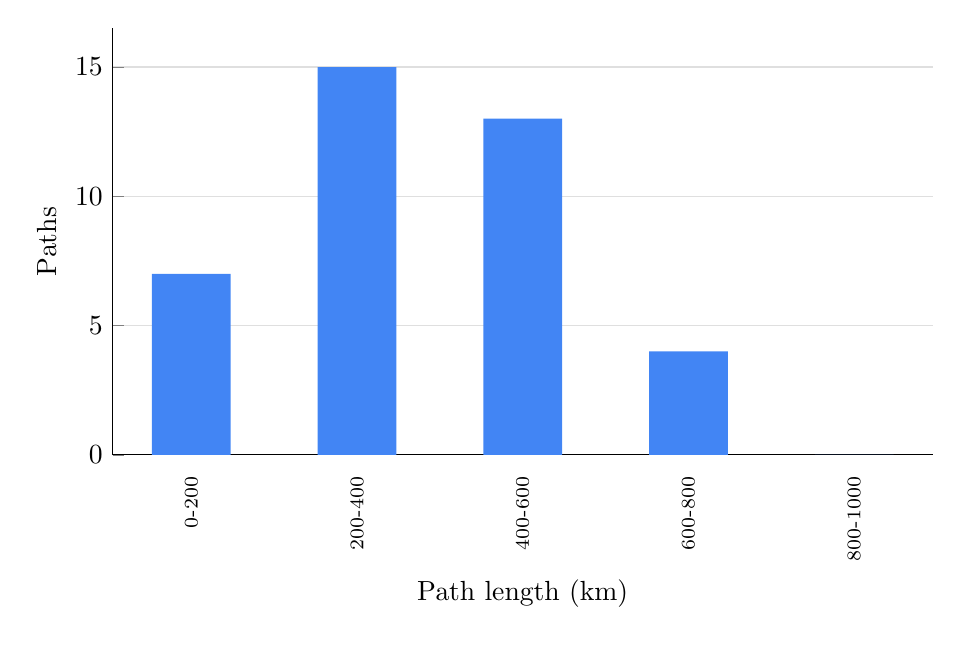
\begin{tikzpicture}
\begin{axis}[
  ybar, bar width=1.000cm, width=12.000cm, height=7cm,
  ymin=0, ymajorgrids, grid style={gray!25}, axis lines*=left,
  enlarge x limits={abs=1.000cm}, xtick=data, major x tick style={draw=none},
  x tick label style={rotate=90, font=\scriptsize, /pgf/number format/1000 sep=},
  legend style={at={(0.5,-0.3)}, anchor=north, legend columns=-1, draw=none},
  ylabel={Paths},
  xlabel={Path length (km)},
  symbolic x coords={0-200,200-400,400-600,600-800,800-1000,1000-1200,1200-1400,1400-1600,1600-1800,1800-2000}]
\addplot[fill={rgb,255:red,66;green,133;blue,244}, draw=none] coordinates {(0-200,7.000) (200-400,15.000) (400-600,13.000) (600-800,4.000) (800-1000,0.000) };
\end{axis}
\end{tikzpicture}\end{center}
\clearpage
\section*{Utilization Entropy}
\begin{center}\begin{adjustbox}{max width=\linewidth}
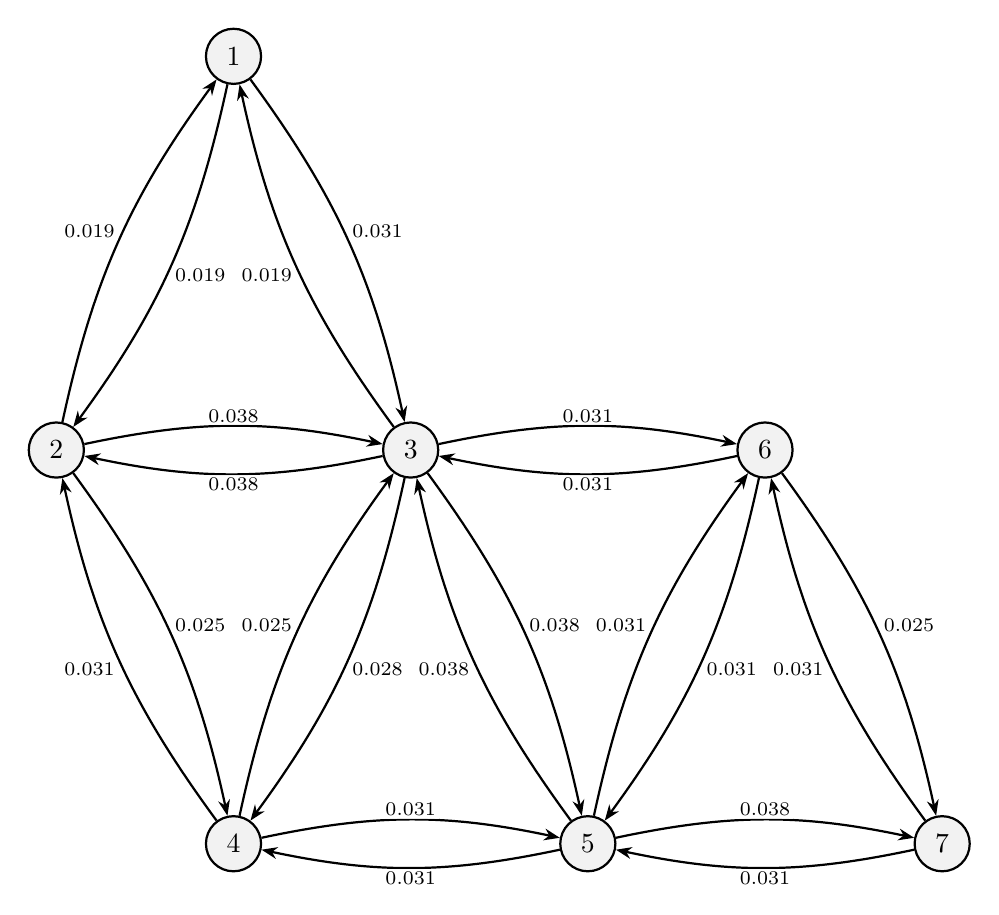
\begin{tikzpicture}[baseline, >={Stealth[length=2mm]},
  netnode/.style={circle, draw, thick, fill=gray!10, minimum size=7mm, inner sep=1pt},
  link/.style={thick},
  linklabel/.style={font=\scriptsize, inner sep=1pt, fill=white, fill opacity=0.85, text opacity=1}]
\node[netnode] (S1) at (2.250,10.000) {1};
\node[netnode] (S2) at (0.000,5.000) {2};
\node[netnode] (S3) at (4.500,5.000) {3};
\node[netnode] (S4) at (2.250,0.000) {4};
\node[netnode] (S5) at (6.750,0.000) {5};
\node[netnode] (S6) at (9.000,5.000) {6};
\node[netnode] (S7) at (11.250,0.000) {7};
\draw[link, ->] (S1) to[bend left=12] node[linklabel, auto] {0.019} (S2);
\draw[link, ->] (S1) to[bend left=12] node[linklabel, auto] {0.031} (S3);
\draw[link, ->] (S2) to[bend left=12] node[linklabel, auto] {0.019} (S1);
\draw[link, ->] (S2) to[bend left=12] node[linklabel, auto] {0.038} (S3);
\draw[link, ->] (S2) to[bend left=12] node[linklabel, auto] {0.025} (S4);
\draw[link, ->] (S3) to[bend left=12] node[linklabel, auto] {0.019} (S1);
\draw[link, ->] (S3) to[bend left=12] node[linklabel, auto] {0.038} (S2);
\draw[link, ->] (S3) to[bend left=12] node[linklabel, auto] {0.028} (S4);
\draw[link, ->] (S3) to[bend left=12] node[linklabel, auto] {0.038} (S5);
\draw[link, ->] (S3) to[bend left=12] node[linklabel, auto] {0.031} (S6);
\draw[link, ->] (S4) to[bend left=12] node[linklabel, auto] {0.031} (S2);
\draw[link, ->] (S4) to[bend left=12] node[linklabel, auto] {0.025} (S3);
\draw[link, ->] (S4) to[bend left=12] node[linklabel, auto] {0.031} (S5);
\draw[link, ->] (S5) to[bend left=12] node[linklabel, auto] {0.038} (S3);
\draw[link, ->] (S5) to[bend left=12] node[linklabel, auto] {0.031} (S4);
\draw[link, ->] (S5) to[bend left=12] node[linklabel, auto] {0.031} (S6);
\draw[link, ->] (S5) to[bend left=12] node[linklabel, auto] {0.038} (S7);
\draw[link, ->] (S6) to[bend left=12] node[linklabel, auto] {0.031} (S3);
\draw[link, ->] (S6) to[bend left=12] node[linklabel, auto] {0.031} (S5);
\draw[link, ->] (S6) to[bend left=12] node[linklabel, auto] {0.025} (S7);
\draw[link, ->] (S7) to[bend left=12] node[linklabel, auto] {0.031} (S5);
\draw[link, ->] (S7) to[bend left=12] node[linklabel, auto] {0.031} (S6);
\end{tikzpicture}
\end{adjustbox}\end{center}

\begin{center}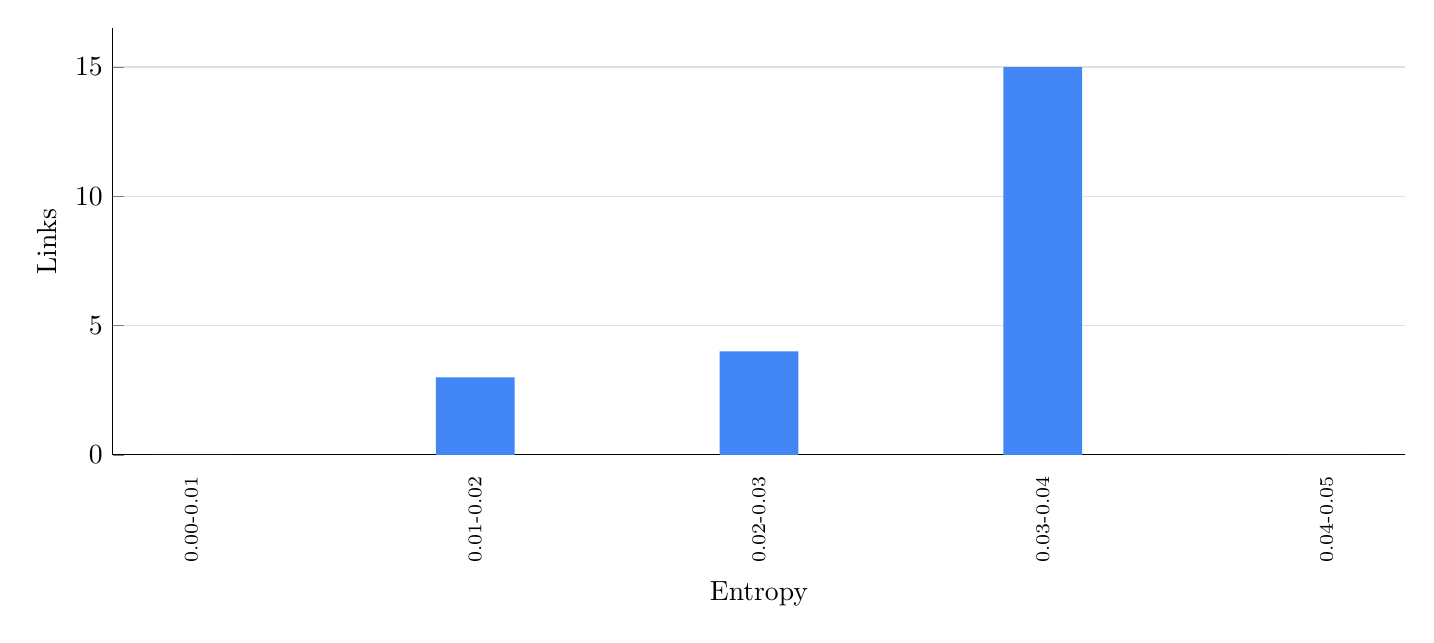
\begin{tikzpicture}
\begin{axis}[
  ybar, bar width=1.000cm, width=18.000cm, height=7cm,
  ymin=0, ymajorgrids, grid style={gray!25}, axis lines*=left,
  enlarge x limits={abs=1.000cm}, xtick=data, major x tick style={draw=none},
  x tick label style={rotate=90, font=\scriptsize, /pgf/number format/1000 sep=},
  legend style={at={(0.5,-0.3)}, anchor=north, legend columns=-1, draw=none},
  ylabel={Links},
  xlabel={Entropy},
  symbolic x coords={0.00-0.01,0.01-0.02,0.02-0.03,0.03-0.04,0.04-0.05,0.05-0.06,0.06-0.07,0.07-0.08,0.08-0.09,0.09-0.10,0.10-0.11,0.11-0.12,0.12-0.13,0.13-0.14,0.14-0.15,0.15-0.16,0.16-0.17,0.17-0.18,0.18-0.19,0.19-0.20,0.20-0.21,0.21-0.22,0.22-0.23,0.23-0.24,0.24-0.25,0.25-0.26,0.26-0.27,0.27-0.28,0.28-0.29,0.29-0.30,0.30-0.31,0.31-0.32,0.32-0.33,0.33-0.34,0.34-0.35,0.35-0.36,0.36-0.37,0.37-0.38,0.38-0.39,0.39-0.40,0.40-0.41,0.41-0.42,0.42-0.43,0.43-0.44,0.44-0.45,0.45-0.46,0.46-0.47,0.47-0.48,0.48-0.49,0.49-0.50,0.50-0.51,0.51-0.52,0.52-0.53,0.53-0.54,0.54-0.55,0.55-0.56,0.56-0.57,0.57-0.58,0.58-0.59,0.59-0.60,0.60-0.61,0.61-0.62,0.62-0.63,0.63-0.64,0.64-0.65,0.65-0.66,0.66-0.67,0.67-0.68,0.68-0.69,0.69-0.70,0.70-0.71,0.71-0.72,0.72-0.73,0.73-0.74,0.74-0.75,0.75-0.76,0.76-0.77,0.77-0.78,0.78-0.79,0.79-0.80,0.80-0.81,0.81-0.82,0.82-0.83,0.83-0.84,0.84-0.85,0.85-0.86,0.86-0.87,0.87-0.88,0.88-0.89,0.89-0.90,0.90-0.91,0.91-0.92,0.92-0.93,0.93-0.94,0.94-0.95,0.95-0.96,0.96-0.97,0.97-0.98,0.98-0.99,0.99-1.00}]
\addplot[fill={rgb,255:red,66;green,133;blue,244}, draw=none] coordinates {(0.00-0.01,0.000) (0.01-0.02,3.000) (0.02-0.03,4.000) (0.03-0.04,15.000) (0.04-0.05,0.000) };
\end{axis}
\end{tikzpicture}\end{center}
\clearpage
\section*{Shannon Entropy}
\begin{center}\begin{adjustbox}{max width=\linewidth}
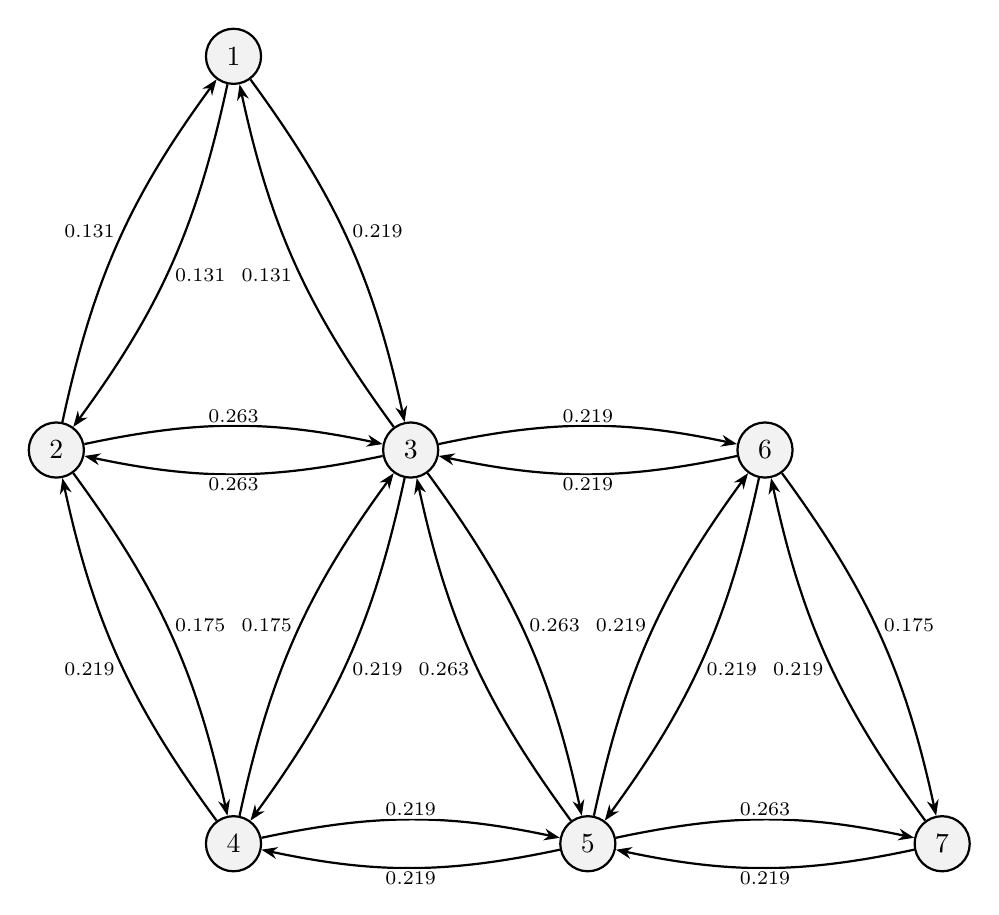
\begin{tikzpicture}[baseline, >={Stealth[length=2mm]},
  netnode/.style={circle, draw, thick, fill=gray!10, minimum size=7mm, inner sep=1pt},
  link/.style={thick},
  linklabel/.style={font=\scriptsize, inner sep=1pt, fill=white, fill opacity=0.85, text opacity=1}]
\node[netnode] (S1) at (2.250,10.000) {1};
\node[netnode] (S2) at (0.000,5.000) {2};
\node[netnode] (S3) at (4.500,5.000) {3};
\node[netnode] (S4) at (2.250,0.000) {4};
\node[netnode] (S5) at (6.750,0.000) {5};
\node[netnode] (S6) at (9.000,5.000) {6};
\node[netnode] (S7) at (11.250,0.000) {7};
\draw[link, ->] (S1) to[bend left=12] node[linklabel, auto] {0.131} (S2);
\draw[link, ->] (S1) to[bend left=12] node[linklabel, auto] {0.219} (S3);
\draw[link, ->] (S2) to[bend left=12] node[linklabel, auto] {0.131} (S1);
\draw[link, ->] (S2) to[bend left=12] node[linklabel, auto] {0.263} (S3);
\draw[link, ->] (S2) to[bend left=12] node[linklabel, auto] {0.175} (S4);
\draw[link, ->] (S3) to[bend left=12] node[linklabel, auto] {0.131} (S1);
\draw[link, ->] (S3) to[bend left=12] node[linklabel, auto] {0.263} (S2);
\draw[link, ->] (S3) to[bend left=12] node[linklabel, auto] {0.219} (S4);
\draw[link, ->] (S3) to[bend left=12] node[linklabel, auto] {0.263} (S5);
\draw[link, ->] (S3) to[bend left=12] node[linklabel, auto] {0.219} (S6);
\draw[link, ->] (S4) to[bend left=12] node[linklabel, auto] {0.219} (S2);
\draw[link, ->] (S4) to[bend left=12] node[linklabel, auto] {0.175} (S3);
\draw[link, ->] (S4) to[bend left=12] node[linklabel, auto] {0.219} (S5);
\draw[link, ->] (S5) to[bend left=12] node[linklabel, auto] {0.263} (S3);
\draw[link, ->] (S5) to[bend left=12] node[linklabel, auto] {0.219} (S4);
\draw[link, ->] (S5) to[bend left=12] node[linklabel, auto] {0.219} (S6);
\draw[link, ->] (S5) to[bend left=12] node[linklabel, auto] {0.263} (S7);
\draw[link, ->] (S6) to[bend left=12] node[linklabel, auto] {0.219} (S3);
\draw[link, ->] (S6) to[bend left=12] node[linklabel, auto] {0.219} (S5);
\draw[link, ->] (S6) to[bend left=12] node[linklabel, auto] {0.175} (S7);
\draw[link, ->] (S7) to[bend left=12] node[linklabel, auto] {0.219} (S5);
\draw[link, ->] (S7) to[bend left=12] node[linklabel, auto] {0.219} (S6);
\end{tikzpicture}
\end{adjustbox}\end{center}

\begin{center}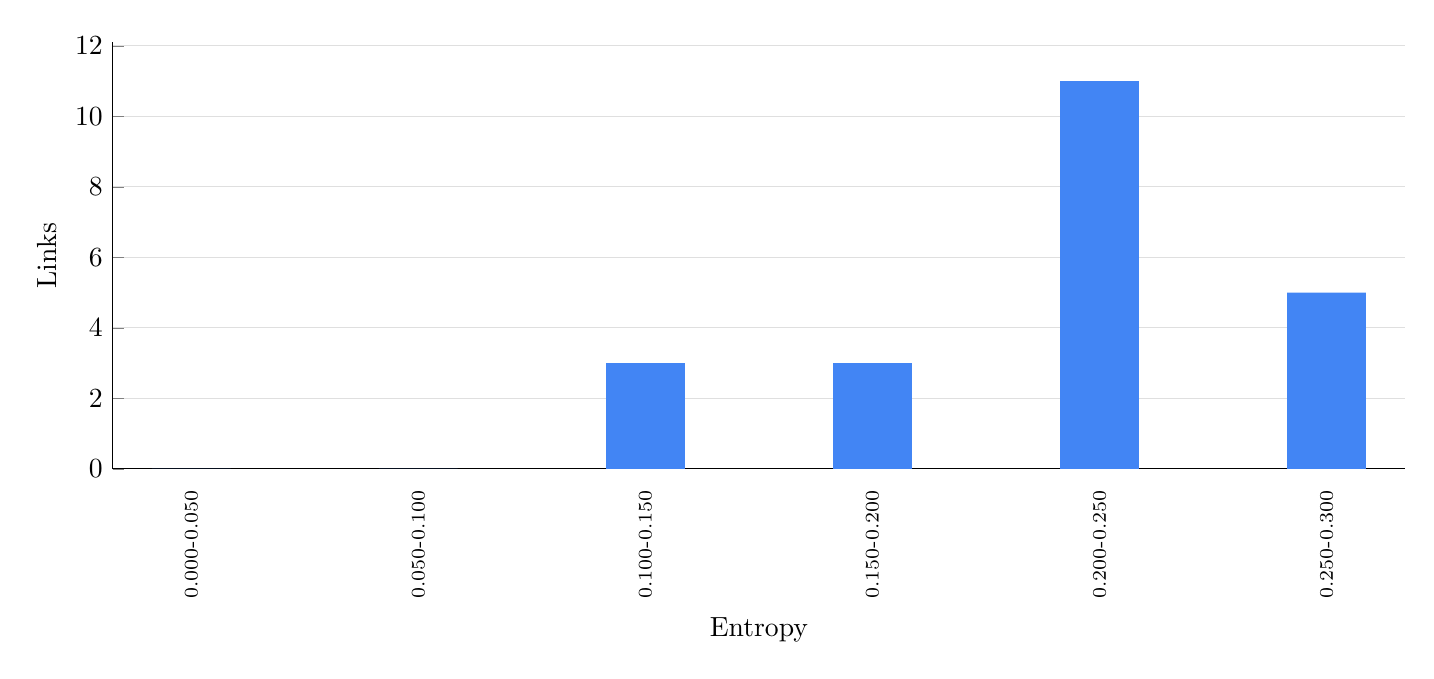
\begin{tikzpicture}
\begin{axis}[
  ybar, bar width=1.000cm, width=18.000cm, height=7cm,
  ymin=0, ymajorgrids, grid style={gray!25}, axis lines*=left,
  enlarge x limits={abs=1.000cm}, xtick=data, major x tick style={draw=none},
  x tick label style={rotate=90, font=\scriptsize, /pgf/number format/1000 sep=},
  legend style={at={(0.5,-0.3)}, anchor=north, legend columns=-1, draw=none},
  ylabel={Links},
  xlabel={Entropy},
  symbolic x coords={0.000-0.050,0.050-0.100,0.100-0.150,0.150-0.200,0.200-0.250,0.250-0.300,0.300-0.350,0.350-0.400,0.400-0.450,0.450-0.500,0.500-0.550,0.550-0.600,0.600-0.650,0.650-0.700,0.700-0.750,0.750-0.800,0.800-0.850,0.850-0.900,0.900-0.950,0.950-1.000}]
\addplot[fill={rgb,255:red,66;green,133;blue,244}, draw=none] coordinates {(0.000-0.050,0.000) (0.050-0.100,0.000) (0.100-0.150,3.000) (0.150-0.200,3.000) (0.200-0.250,11.000) (0.250-0.300,5.000) };
\end{axis}
\end{tikzpicture}\end{center}

\end{document}
